\documentclass[aps,prl,twocolumn, superscriptaddress,groupedaddress,nofootinbib]{revtex4}

\usepackage[utf8]{inputenc}
\usepackage{amsmath}
\usepackage{tikz}
\usepackage{extpfeil}
\usepackage{amsfonts}
\usepackage{amssymb} 
\usepackage{bm}
\usepackage{graphicx}
\usepackage{array}
\usepackage{lipsum}
\usepackage{float}
\usepackage{multirow}
\usepackage{hhline}
\usepackage{tabularx}
\usepackage{subfigure}
\usepackage{graphicx}
\usepackage{afterpage}
\usepackage{longtable}
\usepackage{epstopdf}
\usepackage{amsthm}
\usetikzlibrary{calc}
\let\OLDthebibliography\thebibliography
\renewcommand\thebibliography[1]{
  \OLDthebibliography{#1}
  \setlength{\parskip}{0pt}
  \setlength{\itemsep}{0pt plus 0.3ex}
}

\renewcommand{\thefootnote}{\arabic{footnote}}

\newcommand{\tl}{\text{log}}
\newcommand{\cO}{\mathcal{O}}
\newcommand{\bZ}{\mathbb{Z}}
\newcommand{\bP}{\mathbb{P}}
\newcommand{\bs}[1]{{\color{red}(BS:) #1}}
\newcommand{\jh}[1]{{\color{red}(JH:) #1}}
\newcommand{\cl}[1]{{\color{red}(CL:) #1}}
\newcommand{\jt}[1]{{\color{blue}(JT:) #1}}
\newcommand{\vev}[1]{\langle #1 \rangle}
\newcommand{\ina}{\bar\in}


\begin{document}
\title{Some starter notes on trees}
\author{James Halverson, Cody Long, Benjamin Sung}
\affiliation{Department of Physics, Northeastern University \\ Boston, MA 02115-5000 USA} 

\date{\today}

\begin{abstract}
Abstract here.
\end{abstract}

\maketitle

\section{Technical Considerations}

Let $B$ be a smooth weak Fano toric threefold. Such a variety is naturally
associated with a  fine regular star triangulation (FRST) of a three-dimensional reflexive polytope $\Delta$.
The monomials that may appear in the global sections $f$ and $g$ of the Weierstrass model are 
in one-to-one correspondence with points in the polytopes
\begin{equation} 
P_n := \{m \in \bZ^3 \,\,|\,\, \langle m,v\rangle + n \geq 0 \,\, \forall v \in \Delta \},
\end{equation}
in the cases $n=4,6$, respectively. $\Delta$ is a reflexive polytope because its dual
$\Delta^\circ:=P_1$ is itself a lattice polytope in $\bZ^3$. Then if $x_i$ is the toric
homogeneous coordinate associated with some point $v_i\in \Delta$, the order of vanishing
along $x_i=0$ of some monomial $m_n\in P_n$ is 
\begin{equation}
p_{x_i,m_n} = \langle m,v_i\rangle +n,
\end{equation}
and the overall monomial associated with $m_n$ is $\prod_i x_i^{\langle m_n, v_i\rangle+n}$.
From this the order of vanishings of the monomials along various toric divisors and their intersections
can be read off.

\jh{Filler text will be needed here}

Consider a toric variety $\tilde B$ obtained via a sequence of smooth blowups from the original toric threefold $B$ associated to an FRST of $\Delta$. The vertex associated to any given exceptional divisor is of the form $v_e=\sum a_i v_i$, with non-negative $a_i$, where the points $v_i$ all
lie on some two-face $F$ of $\Delta$. $\tilde B$ also has polytopes $P_n$, which we will call $\tilde P_n$
to distinguish them from the $P_n$ associated to $B$.  Due to the structure of the blowups, for fixed
$n$ $\tilde P_n$ may be obtained by slicing out upper half planes from $P_n$.

\vspace{.5cm}
We will now show that if every exceptional divisor satisfies $\sum a_i \leq 6$, then the generic
Weierstrass model over $\tilde B$ has no $(4,6)$ divisors.

First, note that all vertices of $\tilde B$ are of the form $v=\sum a_i v_i$ with $a_i$ non-negative;
$v$ corresponds to an exceptional divisor if and only if the vector $a_i$ is not a unit vector. This,
together with the definition of $\Delta^\circ$, implies that $\vev{m,v}=\sum a_i \vev{m,v_i} \geq -\sum a_i \geq -6$ for all $v$. This implies that any $m\in \Delta^\circ$ is also an element of $\tilde P_6$; i.e. the associated monomial appears in $g$ of the associated Weierstrass model over $\tilde B$.
Second, consider the unique $m\in \Delta^\circ$ that is dual to a chosen two-face $F$; it satisfies
$\vev{m,v}=-1\,\, \forall v\in F.$ Then for any $v_e=\sum a_i v_i$ that is the sum of multiple vertices in $F$, we have
$\vev{m,v_e}=-\sum a_i < 0$. By the previous argument, $m\in \tilde P_6$, and
rewriting in terms of the power in the exponent we have
\begin{equation}
6 > p_{e,m} \geq 0.
\end{equation}
This implies the monomial $m$ prevents $e=0$ from being a $(4,6)$ divisor. This $m$ does so for
any exceptional divisor built on top of $F$, and for any $F$ there is such an $m$. Therefore, none
of the exceptional divisors of $\tilde B \to B$ are $(4,6)$ divisors.
Third, for any $m\in \Delta^\circ$ and $v \in \Delta$, $m\in \tilde P_6$ by the previous argument
and $\vev{m,v} =-1$ which implies that $g$ vanishes to order $5$ along the associated divisor, and thus it cannot be a $(4,6)$ divisor.

This exhausts the possible types of divisors; therefore any $\tilde B$ obtained in 
this way has no $(4,6)$ divisors.

\vspace{.5cm}
We will now show that to any $\tilde B$ constructed via our method
there is a sequence of smooth toric blowups that together give
$\check B\to \tilde B$ were $\hat B$ has no (4,6) points, curves, or 
divisors. This will be criticall for showing that the general Weierstrass
model over $\tilde B$ is at finite distance in the moduli space
using the Weil-Petersson metric.

Consider any toric curve $C=D_s\cdot D_t \subset \tilde B$. Take $v_s=\sum_i a_{i,s} v_i$ and $v_t=\sum_i a_{i,t} v_i$ and define $a:=\sum_i a_{i,s}$ and $b:=\sum_i a_{i,t}$. Let $F$ be a facet
on which or above which $v_s$ and $v_t$ sit; let $m\in \Delta^\circ$ be the dual to $F$. As an
element of $\tilde P_4$ the associated monomial may be written
\begin{equation}
s^{\vev{m,v_s}+4}t^{\vev{m,v_t}+4}\times \dots,
\end{equation}
and the monomial vanishes to order $\vev{m,v_s}+\vev{m,v_t}+8=-a-b+8$ along $C$,
which must be $\geq 4$ for $C$ to be a $(4,6)$ curve. Therefore $a+b\leq 4$ is necessary for
$C$ to be a $(4,6)$ curve.
Now suppose $C$ is a $(4,6)$ curve that we blow up via $\hat B\to \tilde B$ by
adding an exceptional divisor $v_e = \sum a_i v_i = v_s + v_t$. Then $\sum a_i=a+b$,
which satisfies $\sum a_i\leq 4$ since $C$ is $(4,6)$, but this condition is sufficient to ensure that $\hat B$ has no $(4,6)$ divisors! If $2a+b\leq 4$
or $a+2b\leq 4$ then $\hat B$ may still have a $(4,6)$ curve, but
this blowup process can be iterated until there are no longer
$(4,6)$ curves. So any $\tilde B$ in our construction that has
$(4,6)$ curves admits a sequence of blowups to a smooth toric
threefold with no $(4,6)$ curves or divisors.

We must make a similar argument for $(4,6)$ points. Consider
a point $p=D_s\cdot D_t \cdot D_u \subset \tilde B$, with $v_s$
and $v_t$ as before and $v_u=\sum_i a_{i,u} v_i$ with 
$c:=\sum_i a_{i,u}$. There is a unique facet $F$ above which
or on which $v_{s,t,u}$ all sit, and again $m\in \Delta^\circ$
is the dual to $F$. As an
element of $\tilde P_4$ the associated monomial may be written
\begin{equation}
s^{\vev{m,v_s}+4}t^{\vev{m,v_t}+4}u^{\vev{m,v_u}+4}\times \dots,
\end{equation}
and the monomial vanishes to order $-a-b-c+12$ at $p$.
Therefore $a+b+c\leq 8$ is a necessary condition for $p$ to
be a $(4,6)$ point. If $a+b+c\leq 6$, then the 
blowup of $p$ with $v_e = v_s + v_t + v_u$ has no $(4,6)$
divisors and this type of blowup can be iterated until
either there are no more $(4,6)$ points or there is a $(4,6)$ point
with associated $a, b, c$ satisfying $6<a+b+c\leq 8$.  In
this case the blowup $v_e=v_s+v_t+v_u$ may have a $(4,6)$
divisor. However, a short calculation shows that any positive $a,b,c$
satisfying this bound admits sequences of curve blowups along
$D_s\cdot D_t$, $D_t\cdot D_u$, $D_u\cdot D_s$ that leads to
a threefold base with no $(4,6)$ points, curves, or divisors.


\vspace{.5cm}
Together, these arguments imply that any base $\tilde B$ in our construction has a sequence of smooth toric blowups to another base $\hat B$ (also present in our construction) that has no $(4,6)$ divisors, curves, or points. This means that the elliptic fibration $\hat X \to \hat B$ has canonical singularities, which in turn implies the general Weierstrass model $\tilde X$ over $\tilde B$ also has canonical singularities, since the blowup $\hat B \to \tilde B$ induces a blowup $\hat X\xrightarrow{\phi} \tilde X$. To see that the elliptic fibration $\hat{X}$ has only canonical singularities, we employ a modified version of Nakayama's result as presented in Lemma 3.6 in \cite{Nakayama}. Consider a point $b\in \hat{B}$ and $S$ a smooth surface through $b$. We consider the base change $\hat{X} \times_{\hat{B}} S$ defined by the following pullback diagram.
\begin{center}
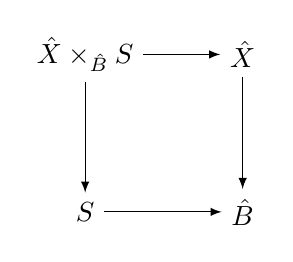
\begin{tikzpicture}[>=latex]
\node (w) at (0,0) {\(\hat{X}\times_{\hat{B}} S\)};
\node (x) at (0,-2) {\(S\)};
\node (y) at (2,0) {\(\hat{X}\)};
\node (z) at (2,-2) {\(\hat{B}\)};
\draw[->] (w) -- (y);
\draw[->] (w) -- (x);
\draw[->] (x) -- (z);
\draw[->] (y) -- (z);
\end{tikzpicture}
\end{center}
\jh{Ben can you give the intuitive sentence about the fiber product, again? The one that made
me and Cody happy? I already forgot.}
We may consider $\hat{X} \times_{\hat{B}} S$ as a Weierstrass model over $S$, which can be thought
of as a restriction within $\hat X$ that gives an elliptic threefold over $S$. By hypothesis, since $\hat{B}$ has no (4,6) points, it follows that $S$ has no (4,6) points and hence the pullback is a minimal Weierstrass model and has rational singularities. By a result of \cite{DefRatSings} on the deformations of rational singularities, it follows that $\hat{X}$ has rational singularities, and since $\hat{B}$ is smooth, it follows that $\hat{X}$ has rational Gorenstein singularities and in particular, at worst canonical singularities. This means that there is a smooth resolution
(not necessarily Calabi-Yau) $X_{s}\xrightarrow{\rho} \hat X$ such that $K_{X_s}=\rho^*(K_{\hat X})+\sum_i a_i E_i$ with all $a_i\geq 0$ and where $E_i$ is an exceptional divisor of $\rho$. Then
we also have a smooth resolution $X_s\xrightarrow{\rho} \hat X\xrightarrow{\phi}\tilde X$ so
that $\tilde X$ also has canonical singularities. To see this, we consider the following diagram 
\begin{center}
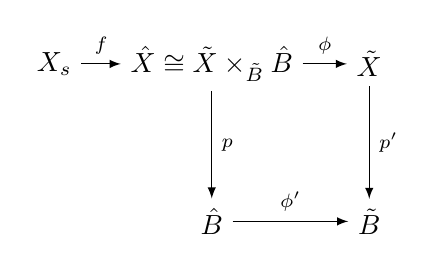
\begin{tikzpicture}[>=latex]
\node (w) at (0,0) {\(\hat{X} \cong \tilde{X}\times_{\tilde{B}} \hat{B}\)};
\node (x) at (0,-2) {\(\hat{B}\)};
\node (y) at (2,0) {\(\tilde{X}\)};
\node (z) at (2,-2) {\(\tilde{B}\)};
\node (a) at (-2,0) {\(X_{s}\)}; 
\draw[->] (w) --  node[auto] {$\scriptstyle \phi$}(y);
\draw[->] (w) -- node[auto] {$\scriptstyle p$}(x);
\draw[->] (x) -- node[auto] {$\scriptstyle \phi'$}(z);
\draw[->] (y) -- node[auto] {$\scriptstyle p'$}(z);
\draw[->] (a) -- node[auto] {$\scriptstyle f$}(w);
\end{tikzpicture}
\end{center}
where $\hat{B}$ is a resolution of $\tilde{B}$ and we take $\hat{X}$ to be induced weierstrass model over $\hat{B}$ from the above pullback diagram. It suffices to show that $R^{\bullet}(\phi\circ f)_{*}(\mathcal{O}_{X_{s}}) \cong \mathcal{O}_{\tilde{X}}$. By hypothesis, $R^{\bullet}f_{*}(\mathcal{O}_{X_{s}}) \cong \mathcal{O}_{\hat{X}}$ and $R^{\bullet}\phi'_{*}(\mathcal{O}_{\hat{B}}) \cong \mathcal{O}_{\tilde{B}}$. Applying the Grothendieck spectral sequence, we have that $R^{\bullet}(\phi\circ f)_{*}(\mathcal{O}_{X_{s}}) \cong R^{\bullet}\phi_{*}(\mathcal{O}_{\hat{X}})$. Since $p'$ in particular, is a flat morphism, and flatness is stable under base change, $p$ is also a flat morphism, and in particular, we have the induced isomorphism $p'^{*}R^{\bullet}\phi'_{*}\mathcal{O}_{\hat{B}} \xrightarrow{\sim} R^{\bullet}\phi_{*}p^{*}\mathcal{O}_{\hat{B}}$. It follows that $R^{\bullet}\phi_{*}(\mathcal{O}_{\hat{X}}) \cong R^{\bullet}\phi_{*}p^{*}(\mathcal{O}_{\hat{B}})\cong p'^{*}R^{\bullet}\phi'_{*}\mathcal{O}_{\hat{B}}\cong p'^{*}\mathcal{O}_{\tilde{B}} \cong \mathcal{O}_{\tilde{X}}$ as desired. Thus, it follows that $\tilde{X}$ also has rational gorenstein singularities.
Any F-theory model on $\tilde{X}$ in our construction therefore has canonical
singularities, and by results of Hayakawa \cite{Hayakawa} and Wang \cite{Wang}
they are all at finite distance from one another in the Weil-Petersson metric on moduli space.

\indent

\section{Gauge Configurations}
We now embark on a combinatorial study of locality of non-Higgsable clusters on intersecting divisors. Indeed, we first observe trivially that sufficiently tall trees on one simplex may induce non-Higgsable clusters on another simplex with some relative height difference that could be quantitatively analyzed. Let $v_{1}$, $v_{2}$, and $v_{3}$ denote three rays forming a smooth, rational, polyhedral cone, and define $v_{e} \equiv av_{1} + bv_{2} + cv_{3}$ with $(a,b,c) \in \mathbb{Z}^{3}_{\geq 0}$. Define $H_{n,e}$ to be the hyperplane defined by $\langle m,v_{e} \rangle = -n$ and define $H_{n,i}$ to be the upper half-planes defined by $\langle m,v_{i} \rangle \geq -n$ for $i = 1,2,3$. We wish to study the region defined by $H \equiv H_{n,e} \bigcap\limits_{i}H_{n,i}$. 

We first show that there exists a finite number of integral points in $H$. Consider the equation given by $\langle m, v_{e} \rangle = a\langle m, v_{1} \rangle + b\langle m, v_{2} \rangle + c\langle m, v_{3} \rangle = -n$. As the tuple $(a,b,c)$ are strictly positive, it easily follows from the above inequalities, that $\langle m, v_{i} \rangle$ are also bounded above. Thus, we consider the integral solution set to the matrix inequality 
\begin{equation}
  \begin{pmatrix}
  -n \\ -n \\ -n
  \end{pmatrix}
  \begin{array}{@{}c@{}}
 {} \\ \leq \\ {}
  \end{array}
  \begin{pmatrix}
     {} & v_{1} & {} \\
    {} & v_{2} &{} \\
    {}  & v_{3} & {}
  \end{pmatrix}
  \begin{pmatrix}
    {} \\ m \\ {} 
  \end{pmatrix}
  \begin{array}{@{}c@{}}
    {} \\ \leq \\ {}
  \end{array}
  \begin{pmatrix}
    n_{1} \\ n_{2} \\ n_{3}
  \end{pmatrix}
\end{equation}
As the vectors $v_{i}$ form a basis for $\mathbb{Z}^{3}$ by hypothesis, it follows easily that there exists only finitely many integral solutions to the above matrix inequality, and hence we are done.

We now give a sufficient condition for bounding hyperplanes to eliminate points on the hyperplane $H_{n,e}$. Let $v_{e}$ and the $v_{i}$ be as defined above, and define $v_{i}' \equiv a_{i}v_{1} + b_{i}v_{2} + c_{i}v_{3}$ for positive integers $a_{i}$, $b_{i}$, and $c_{i}$ such that $v_{1}' + v_{2}' + v_{3}' = v_{e}$. We construct three smooth torus-equivariant blowups along the toric curves given by the edges $(v_{e},v_{i}')$ for $i = 1,2,3$. The resulting hyperplane inequalities given by the vertices $v_{e} + v_{i}'$ yield the condition $\langle m, 3v_{e} + v_{1}' + v_{2}' + v_{3}'\rangle = \langle m, 4v_{e} \rangle \geq -3n$. Thus, we find that $\langle m, v_{e} \rangle \geq -\frac{3}{4}n$ and hence there does not exist integral points on the hyperplane $H_{n,e}$.

\subsection{Minimal Vanishing From Resolution}
\cl{to discuss notation}
A blow-up on an $n$-face $F_n \subset \Delta^\circ$ ($n = 0, 1, 2$) will induce a minimal order of vanishing in $f$ and $g$ along the divisors corresponding to the points involved in the blow-up, as well as any of the points interior to any higher codimension faces bounded by $F_n$. In this section we derive this by consider blow-ups along faces of each dimension.
\subsubsection{Points interior to facets}
First, we consider a point $p$ interior to a facet $F$, with corresponding divisor $D_p$, and homogenous coordinate $x_p$. To check for non-Higgsable 7-branes on $D_p$, we check for the absence of any monomials $m_n$ such that $\langle m_n, p \rangle = -n$, for $n = 4,6$. Define the lattice polytope corresponding to the sections of degree $\mathcal{O}(-n K_B)$ as $\Delta_n$. We note that all vertices of $\Delta_n$ take the form $nm_i$, where the $m_i$ are the vertices of $\Delta$. Recall that there exists a vertex $m\subset \Delta$ dual to $F: \langle m, F \rangle = -1$. Let the vertices that are not $m$ be $\hat{m}_j$. Since $\langle m, p \rangle = -1$, and $\langle \hat{m}_j, p \rangle \geq 0$, it is clear that $\langle n\,m, p \rangle = -n$, and $\langle n\,\hat{m}_j, p \rangle \geq 0$. Therefore the linear function $\langle p, \cdot \, \rangle$ is minimized at $m$, and is strictly increasing when moving from $m$ to any other vertex, and therefore strictly increasing when moving away from $m$ in any direction. Therefore, $m$ is the only monomial satisfying $\langle p, \cdot\, \rangle = -n$. Therefore, before resolution there is a single monomial in $f$ ($g$), which is degree zero in $x_p$, and corresponds to a vertex in $\Delta_4$ ($\Delta_6$). The existence of these monomials obstructs the existence of non-Higgsable 7-branes along $D_p$.

Now let us consider a resolution, with exceptional divisor $D_e = \sum a_i D_i$, where $a_i \in \{ 0, 1\}$, and the $D_i$ correspond to points $v_i$ on $F$, which can be vertices, points interior to edges that bound $F$, or points strictly interior to $F$. For the blow-up to be non-trivial either two or three of the $a_i$ are non-zero. This blow-up introduces a hyperplane that further cuts $\Delta_n$ to $\tilde{\Delta}_n$. In particular, we consider the effect on the monomial $n\, m$. First, let us note that if we have an $m \in \Delta$ such that $\langle m, p \rangle = -1$, where $p$ is in the strict interior of a facet $F$, then $\langle m, v_i \rangle = -1$ for all other $v_i \in F$. To see this, consider a triangulation of $F$ using the vertices of $F$ as vertices in the triangulation. Then all other points lie within the simplices of the triangulation. Let $p$ lie within a simplex generated by the points $\{v_1, v_2, v_3\}$. Then we can write $ p = a_1 v_1 + a_2 v_2 + (1 -a_1 - a_2) v_3$, where $0 < a_i < 1$. Therefore, we have $-1 = a_1 \langle m, v_1\rangle + a_2 \langle m, v_2\rangle+ (1 - a_1 - a_2) \langle m, v_3\rangle$. From the reflexivity of $\Delta^\circ$ we have $\langle v_i, m \rangle \geq -1$. Assume that $\langle m, v_1\rangle > -1$. We then have $-1 > -a_1+ a_2 \langle m, v_2\rangle+ (1 - a_1 - a_2) \langle m, v_3\rangle > -a_1 -a_2 - (1 -a_1 - a_2) = -1$, which is a contradiction. One can repeat this argument to see that all of the the $\langle m, v_i\rangle = -1$. 

Now we take the inner product of $n\, m$ with $v \equiv \sum_i a_i v_i$, we have $\langle n\, m, v \rangle = -1$. Then $\langle m, v\rangle -n \sum_i v_i$, which must satisfy $\langle m, v\rangle -n \sum_i v_i \geq -n$ for $m$ to be an allowed point in $\tilde{\Delta}_n$. However, a non-trivial blow-up have $\sum_i v_i > 1$, and therefore the blowup cuts out the point $m$ from $\tilde{\Delta}_n$. Applying this to $\Delta_f$ and $\Delta_g$, we can see that after the resolution both $f$ and $g$ will vanish to at least order one along $x_p$. Therefore any blow-up along any points in $F$ will automatically introduce at least a type $II$ singularity along all divisors corresponding to points in the strict interior of $F$.
\subsubsection{Points interior to edges}
We now perform a similar analysis for a divisor $D_p$ corresponding to a point $p$ with homogeneous coordinate $x_p$, and is interior to an edge $E$. In this case, the dual to $p$ in $\Delta$ under $\langle p, \cdot \, \rangle = -1$ is an entire edge of points $E_\Delta \in \Delta$, bounded by two vertices which we label $m_1$ and $m_2$. $m_1$ and $m_2$ are vertices in $\Delta$, and therefore $n m_1$ and $n m_2$ are vertices in $\Delta_n$, which bound an edge $E_{n} \subset \Delta_n$. Every point $m^i_{E_n} \in E_{n}$ then satisfies $\langle m^i_{E_n} , p \rangle = -n$. Since all other vertices $\hat{m}_j \neq m_1, m_2$ in $\Delta$ satisfy $\langle \hat{m}_j, p\rangle \geq 0$, then all vertices $n \hat{m}_j \neq n m_1, n m_2$ of $\Delta_n$ satisfy $\langle n \hat{m}_j, p\rangle \geq 0$. The linear function $\langle p, \cdot \, \rangle$ is then minimized along $E_n$ and strictly increasing when moving away from $E_n$, and therefore the only points $m_n$ in $\Delta_n$ satisfying $ \langle p, \cdot \, \rangle = -n$ are the $m^i_{E_n}$. In a similar fashion to the $p \in F$ case one can show that $\langle m^i_{E_n}, v_i \rangle = -n$ for all points $v_i$ on $E$. 

We now perform a blow-up using two points $v_1$ and $v_2$ on $E$, introducing a new ray $v = v_1 + v_2$ and corresponding exceptional divisor $D_v = D_1 +D_2$, where the $D_i$ correspond to the $v_i$. Again, this resolution will cut points out of $\Delta_n$ by introducing an additional hyperplane constraint. We consider the effect on the points $m^i_{E_n}$, which correspond to the non-trivial monomials in $\mathcal{O}(-n K_B)$ that are degree zero in $x_p$. We have $\langle m^i_{E_n}, v \rangle = -2 n$. However, this violates $\langle m^i_{E_n}, v \rangle \geq -n$, and therefore the resolution cuts out all degree zero monomials in $x_p$. Therefore any resolution along $E$ will introduce at least a type $II$ singularity along each divisor corresponding to a point on the strict interior of $E$. \cl{stopping here, I don't think there's a direct continuation of this argument to vertices}

\subsection{Monomial Chopping}

For many of the analyses in this paper we use small
lemmas about when monomials of certain types are chopped out. We would 
like to prove them here.

\begin{proof}
Suppose $h_v \leq 6/n$, $\forall v=av_1+bv_2+cv_3 \ina \Delta^\circ$, where
the leaf height $h_v=a+b+c$. Then  since $m\cdot v_i\geq -1 \forall v\in \Delta^\circ$,
nm
\end{proof}

\bibliography{refs}

\end{document}


%%% Local Variables:
%%% mode: latex
%%% TeX-master: t
%%% End:
